% QUESTAO
A figura abaixo é composta de um retângulo cujos lados medem $x+4$ e $2x+3$.
\begin{center}
	\vspace{-3mm}
	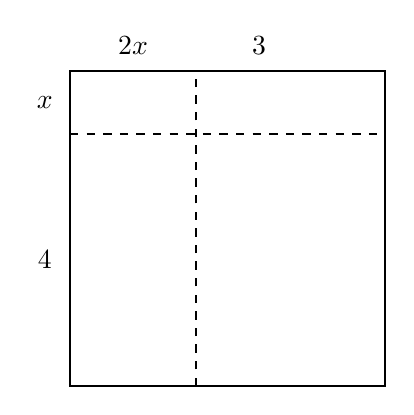
\begin{tikzpicture}[scale=0.8]
	\draw[thick] (0,0) rectangle (5,5);
	\draw[thick, dashed] (2,0)--(2,5) (0,4)--(5,4);
	\node at (-0.4,2) {$4$};
	\node at (-0.4,4.5) {$x$};
	\node at (1,5.4) {$2x$};
	\node at (3,5.4) {$3$};
	\end{tikzpicture}
	\vspace{-3mm}
\end{center}
Escreva um polinômio reduzido que represente a área dessa figura.

% ALTERNATIVAS 7
$A=2x^2+11x+12$
$A=x^2+8x+12$
$A=2x^2+3x+7$
$A=3x^2+7x+10$
$A=2x^2+3x+4$



